\documentclass[3p,times,procedia]{elsarticle}


\flushbottom

%% The `ecrc' package must be called to make the CRC functionality available
\usepackage{ecrc}
%\usepackage{amsmath}


%% The ecrc package defines commands needed for running heads and logos.
%% For running heads, you can set the journal name, the volume, the starting page and the authors

%% set the volume if you know. Otherwise `00'
\volume{00}

%% set the starting page if not 1
\firstpage{1}

%% Give the name of the journal
\journalname{24th EURO Working Group on Transportation Meeting, EWGT 2021, 8-10 September 2021, Aveiro, Portugal}

%% Give the author list to appear in the running head
%% Example \runauth{C.V. Radhakrishnan et al.}
\runauth{J. Raimbault and M. Batty}

%% The choice of journal logo is determined by the \jid and \jnltitlelogo commands.
%% A user-supplied logo with the name <\jid>logo.pdf will be inserted if present.
%% e.g. if \jid{yspmi} the system will look for a file yspmilogo.pdf
%% Otherwise the content of \jnltitlelogo will be set between horizontal lines as a default logo

%% Give the abbreviation of the Journal.
\jid{trpro}

%% Give a short journal name for the dummy logo (if needed)
%\jnltitlelogo{Transportation Research}

%% Hereafter the template follows `elsarticle'.
%% For more details see the existing template files elsarticle-template-harv.tex and elsarticle-template-num.tex.

%% Elsevier CRC generally uses a numbered reference style
%% For this, the conventions of elsarticle-template-num.tex should be followed (included below)
%% If using BibTeX, use the style file elsarticle-num.bst

%% End of ecrc-specific commands
%%%%%%%%%%%%%%%%%%%%%%%%%%%%%%%%%%%%%%%%%%%%%%%%%%%%%%%%%%%%%%%%%%%%%%%%%%

%% The amssymb package provides various useful mathematical symbols

\usepackage{amssymb}
%% The amsthm package provides extended theorem environments
%% \usepackage{amsthm}

%% The lineno packages adds line numbers. Start line numbering with
%% \begin{linenumbers}, end it with \end{linenumbers}. Or switch it on
%% for the whole article with \linenumbers after \end{frontmatter}.
%% \usepackage{lineno}

%% natbib.sty is loaded by default. However, natbib options can be
%% provided with \biboptions{...} command. Following options are
%% valid:

%%   round  -  round parentheses are used (default)
%%   square -  square brackets are used   [option]
%%   curly  -  curly braces are used      {option}
%%   angle  -  angle brackets are used    <option>
%%   semicolon  -  multiple citations separated by semi-colon
%%   colon  - same as semicolon, an earlier confusion
%%   comma  -  separated by comma
%%   numbers-  selects numerical citations
%%   super  -  numerical citations as superscripts
%%   sort   -  sorts multiple citations according to order in ref. list
%%   sort&compress   -  like sort, but also compresses numerical citations
%%   compress - compresses without sorting
%%
\biboptions{authoryear}

% \biboptions{}

% if you have landscape tables
\usepackage[figuresright]{rotating}
%\usepackage{harvard}
% put your own definitions here:x
%   \newcommand{\cZ}{\cal{Z}}
%   \newtheorem{def}{Definition}[section]
%   ...

% add words to TeX's hyphenation exception list
%\hyphenation{author another created financial paper re-commend-ed Post-Script}

% declarations for front matter

\usepackage[bookmarks=false]{hyperref}
    \hypersetup{colorlinks,
      linkcolor=blue,
      citecolor=blue,
      urlcolor=blue}

\usepackage{multicol}




\begin{document}
\begin{frontmatter}

%% Title, authors and addresses

\title{Scientific workflow systems as platforms to integrate modular urban transportation models}

\author[a,b,c]{Juste Raimbault\corref{cor1}}
\author[a]{Mike Batty}

\address[a]{CASA, University College London, London, United Kingdom}
\address[b]{UPS CNRS 3611 Complex Systems Institute, Paris, France}
\address[c]{UMR CNRS 8504 G{\'e}ographie-cit{\'e}s, Paris, France}

\begin{abstract}
Large scale urban transportation models such as four-step models require the integration of heterogenous data and the coupling of sub-models which can already be consequent in terms of complexity. Therefore, such integrated models are difficult to transfer, reproduce, and validate. We propose a modular and reproducible approach based on scientific workflow systems to build and validate such models. We illustrate it by coupling different open-source components within workflows to construct a four-step transportation model applied to all functional urban areas in the UK, and discuss its application to health indicators within public transport in the context of the COVID-19 crisis.
\end{abstract}

\begin{keyword}
Urban transport models \sep Scientific workflow systems \sep Modularity \sep Reproducibility
\end{keyword}
\cortext[cor1]{Corresponding author.}
\end{frontmatter}

\email{j.raimbault@ucl.ac.uk}

%%
%% Start line numbering here if you want
%%
% \linenumbers

%% main text

%\enlargethispage{-7mm}
%\section{Introduction}

\cite{argent2004overview} : components

\cite{lovelace2020open}

\cite{cheetham2021determining}

\cite{leung2021real}

\cite{chen2021effects}

quant paper: \cite{batty2021new}

\cite{usher2019software}

\cite{horl2021integrating}

\cite{horl2020reproducible}

% https://scholar.google.com/scholar?hl=fr&as_sdt=0%2C5&q=covid+transmission+public+transport&oq=covid+transmission+publi#d=gs_qabs&u=%23p%3D9Ng_8CQbmYYJ


Urban transportation models such as four-step models, and more generally land-use transport interaction models \citep{wegener2004land}, require the integration of heterogenous data and the coupling of various submodules with possibly high levels of complexity. This raises issues on the one hand for their implementation, transferability and reproducibility, and on the other hand for their validation which requires large scale numerical experiments to validate the submodules and the whole models \citep{lee1973requiem,batty2014can}. This work proposes to tackle both issues by leveraging modularity and transparency for the construction of large urban models in a modular way, using scientific workflow systems \citep{barker2007scientific} to couple the different components of models and to launch numerical experiments for their validation.

More particularly, we demonstrate this approach by building a modular four-step multimodal transportation model using only open-source projects. We couple together the MATSim model (MATSim Community \citep{horni2016multi}) to simulate the transportation system, the SPENSER model (University of Leeds, \url{https://github.com/nismod/microsimulation}) for the generation of synthetic population, the QUANT model (University College London \citep{milton2019accelerating}) to estimate spatial interactions, and the spatialdata library (OpenMOLE Community \citep{raimbault2020scala}) for data preparation. The model parts are embedded as docker containers into the DAFNI facility (\url{https://dafni.ac.uk/}), which workflow system is used to couple them and build the integrated model. DAFNI provides a scientific workflow system for model integration and coupling, direct access to relevant open datasets, visualisation functionalities, and access to a High Performance Computing infrastructure. We show in Fig.~\ref{fig:fig1} the workflow constructed with the interactive workflow builder within the platform, and an example of visualisation of model outputs.


%%%%%%%%%%%%
\begin{figure}[t]\vspace*{4pt}
\begin{center}
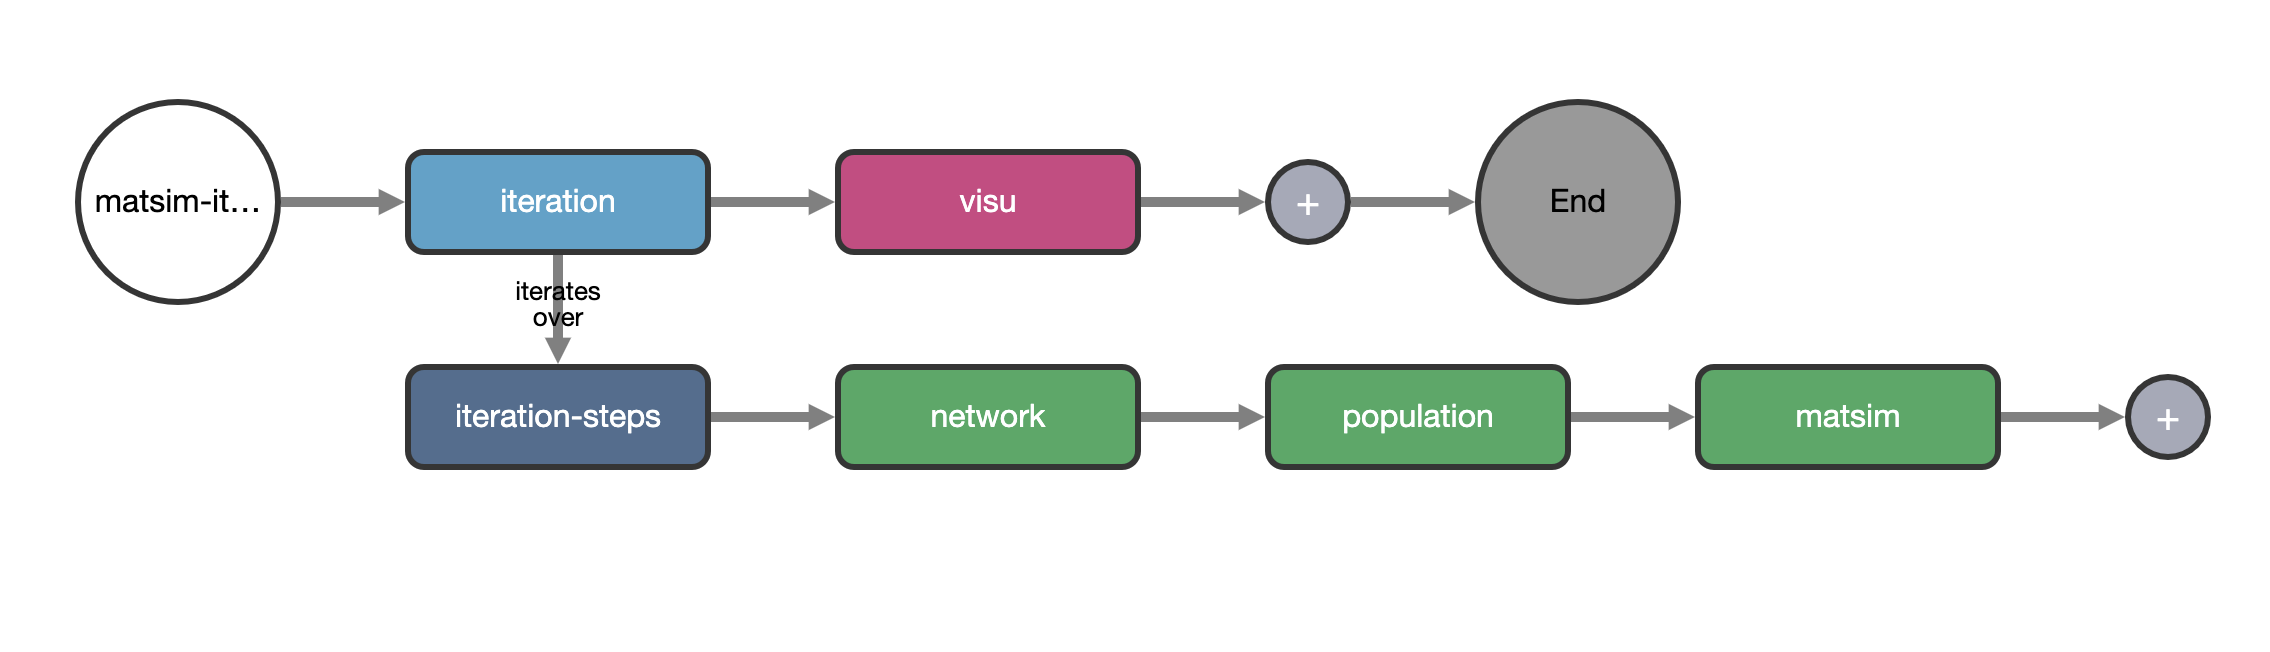
\includegraphics[width=0.7\linewidth]{figures/matsim-iterations_workflow.png}\\
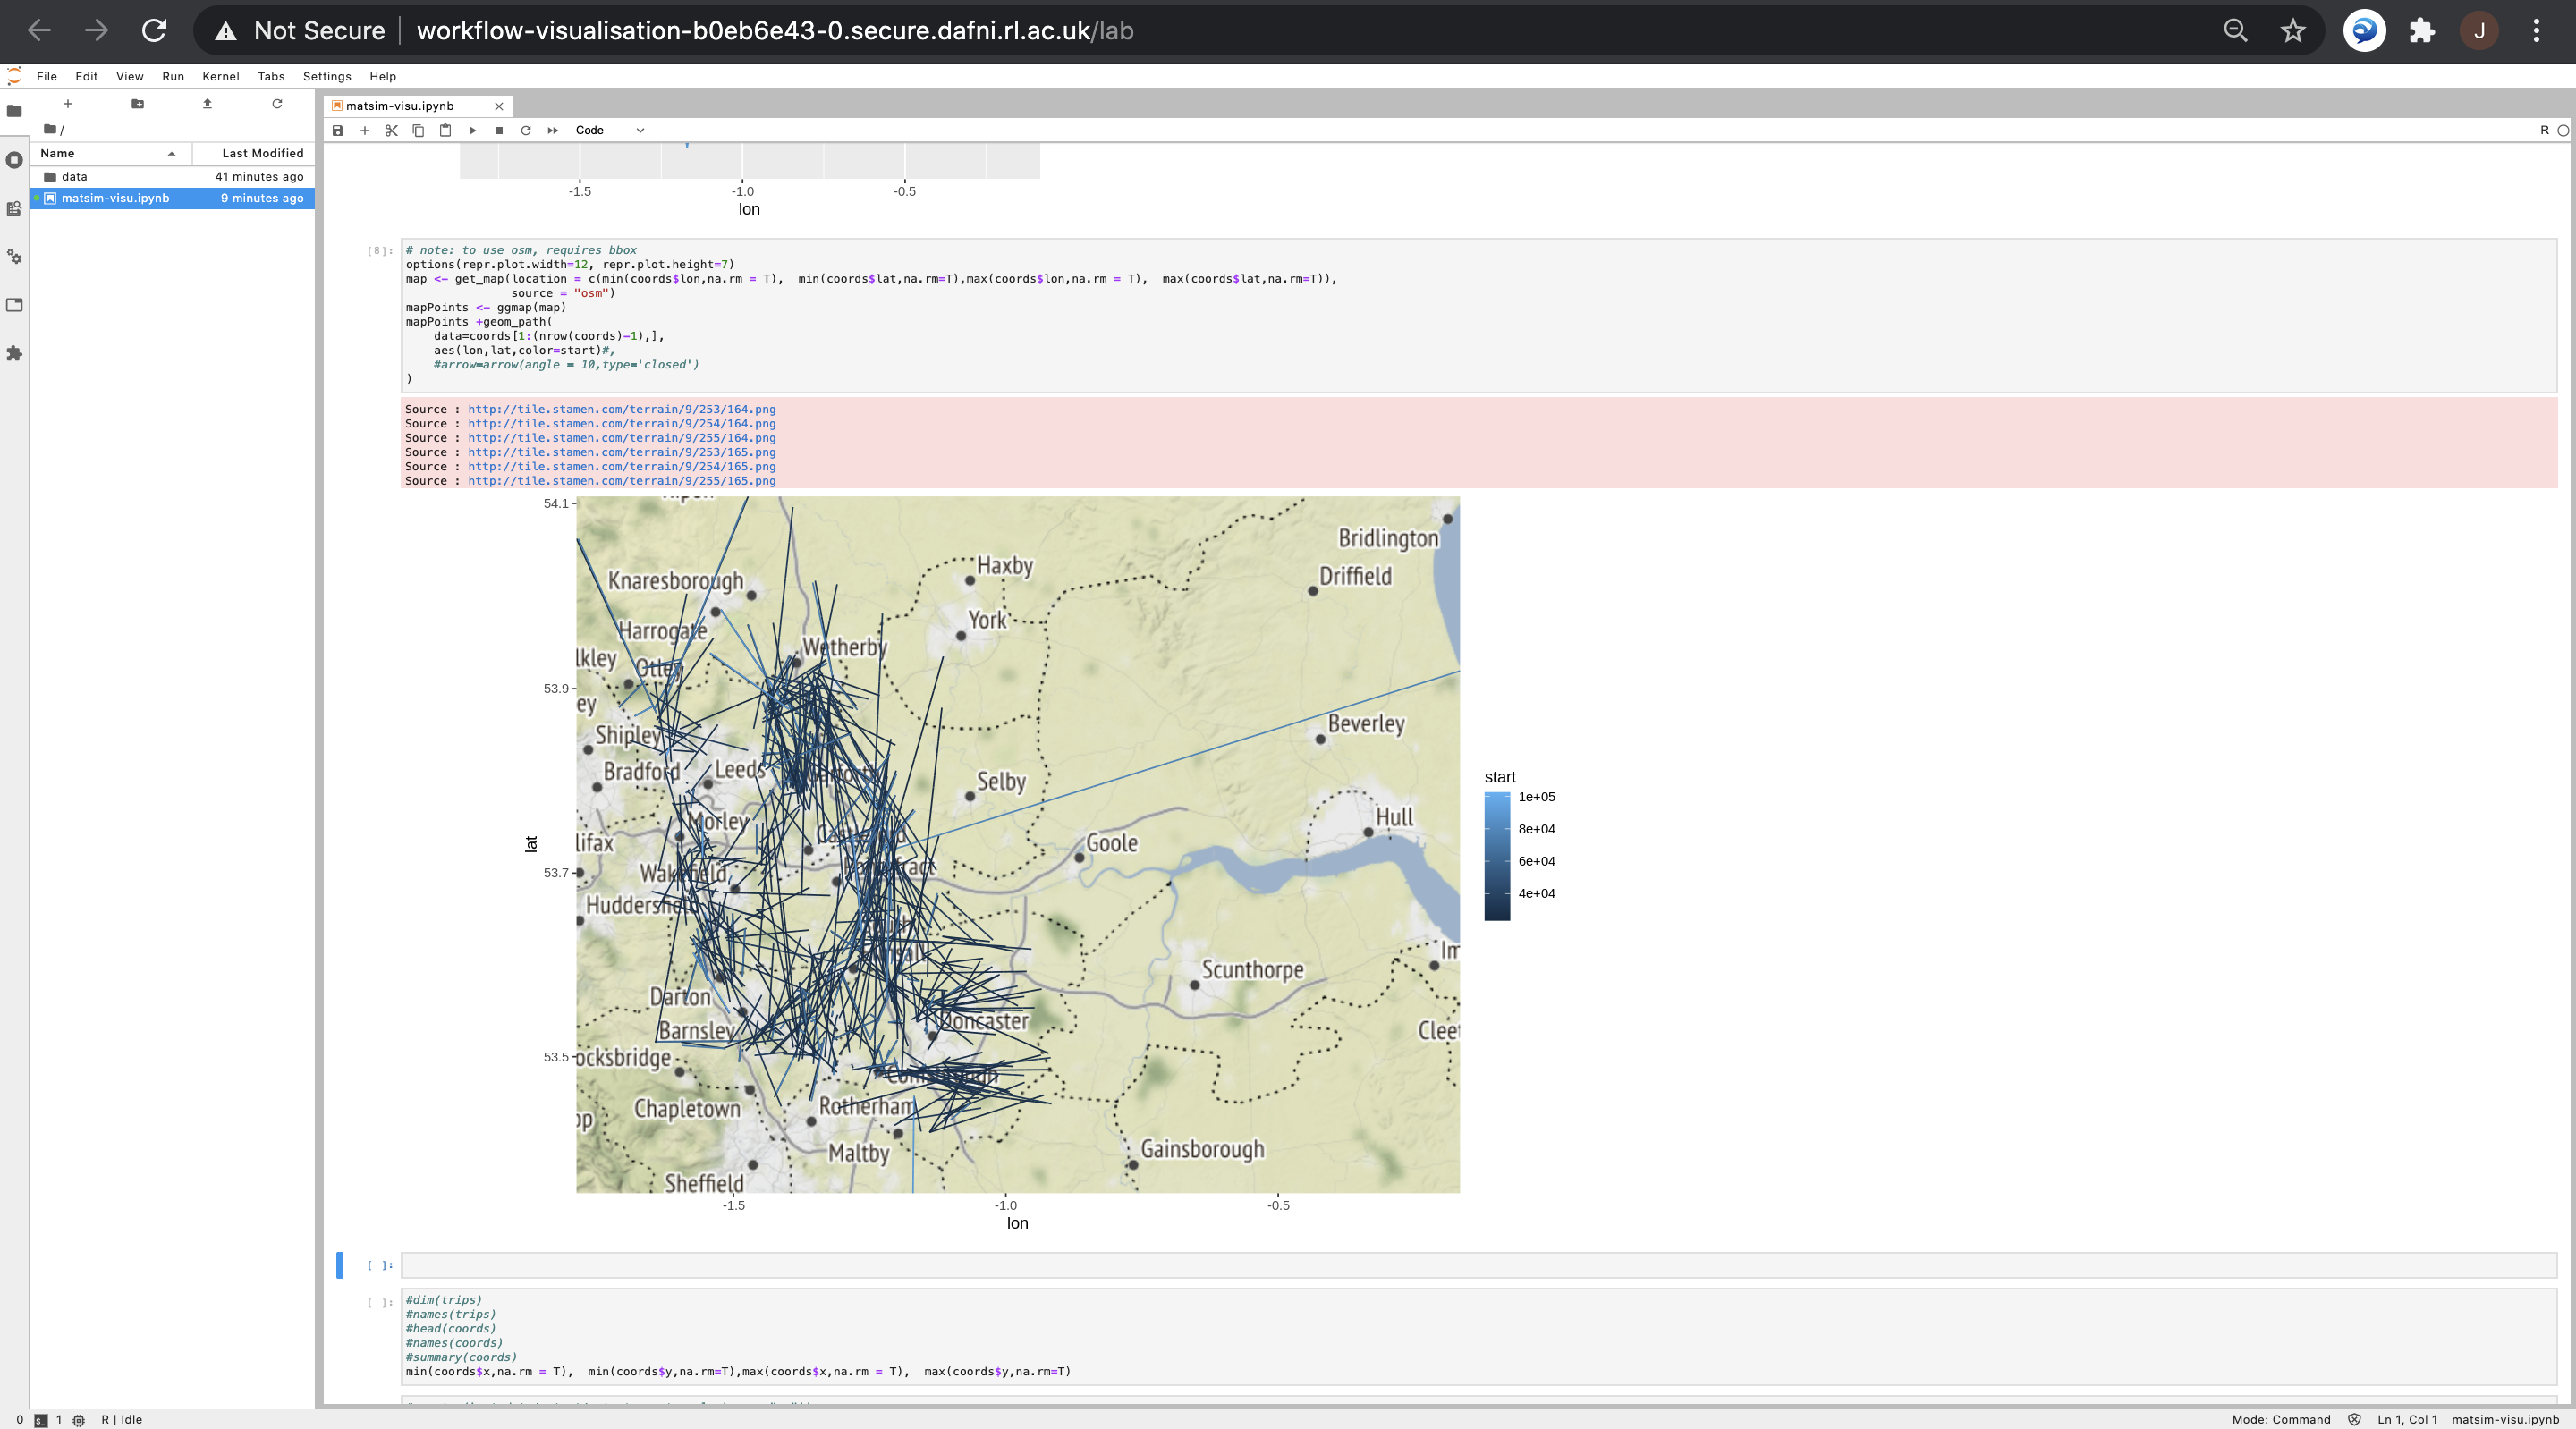
\includegraphics[width=0.7\linewidth]{figures/visu-trips-Leeds.png}	
\end{center}
\caption{Construction of the transport model using the DAFNI workflow system. \textit{(Top)} DAFNI workflow including model steps and a computational experiment (Monte Carlo simulations); \textit{(Bottom)} Example of visualisation of model output (MATSim generated trips) within the DAFNI platform.\label{fig:fig1}}
\end{figure}
%%%%%%%%%%%%




The model is run on the largest functional urban areas (following the definition of \cite{florczyk2019ghsl}) in the UK. We show first results of numerical experiments studying the role of stochasticity on model outputs, for example in Fig.~\ref{fig:fig2} for the statistical distribution of trip departure times (these are iteratively evolved by agents in the MATSim model) for a given urban area. We also show in Fig.~\ref{fig:fig2} the distribution of car trip distances in the different urban areas.


%%%%%%%%%%%%
\begin{figure}[t]\vspace*{4pt}
\begin{center}
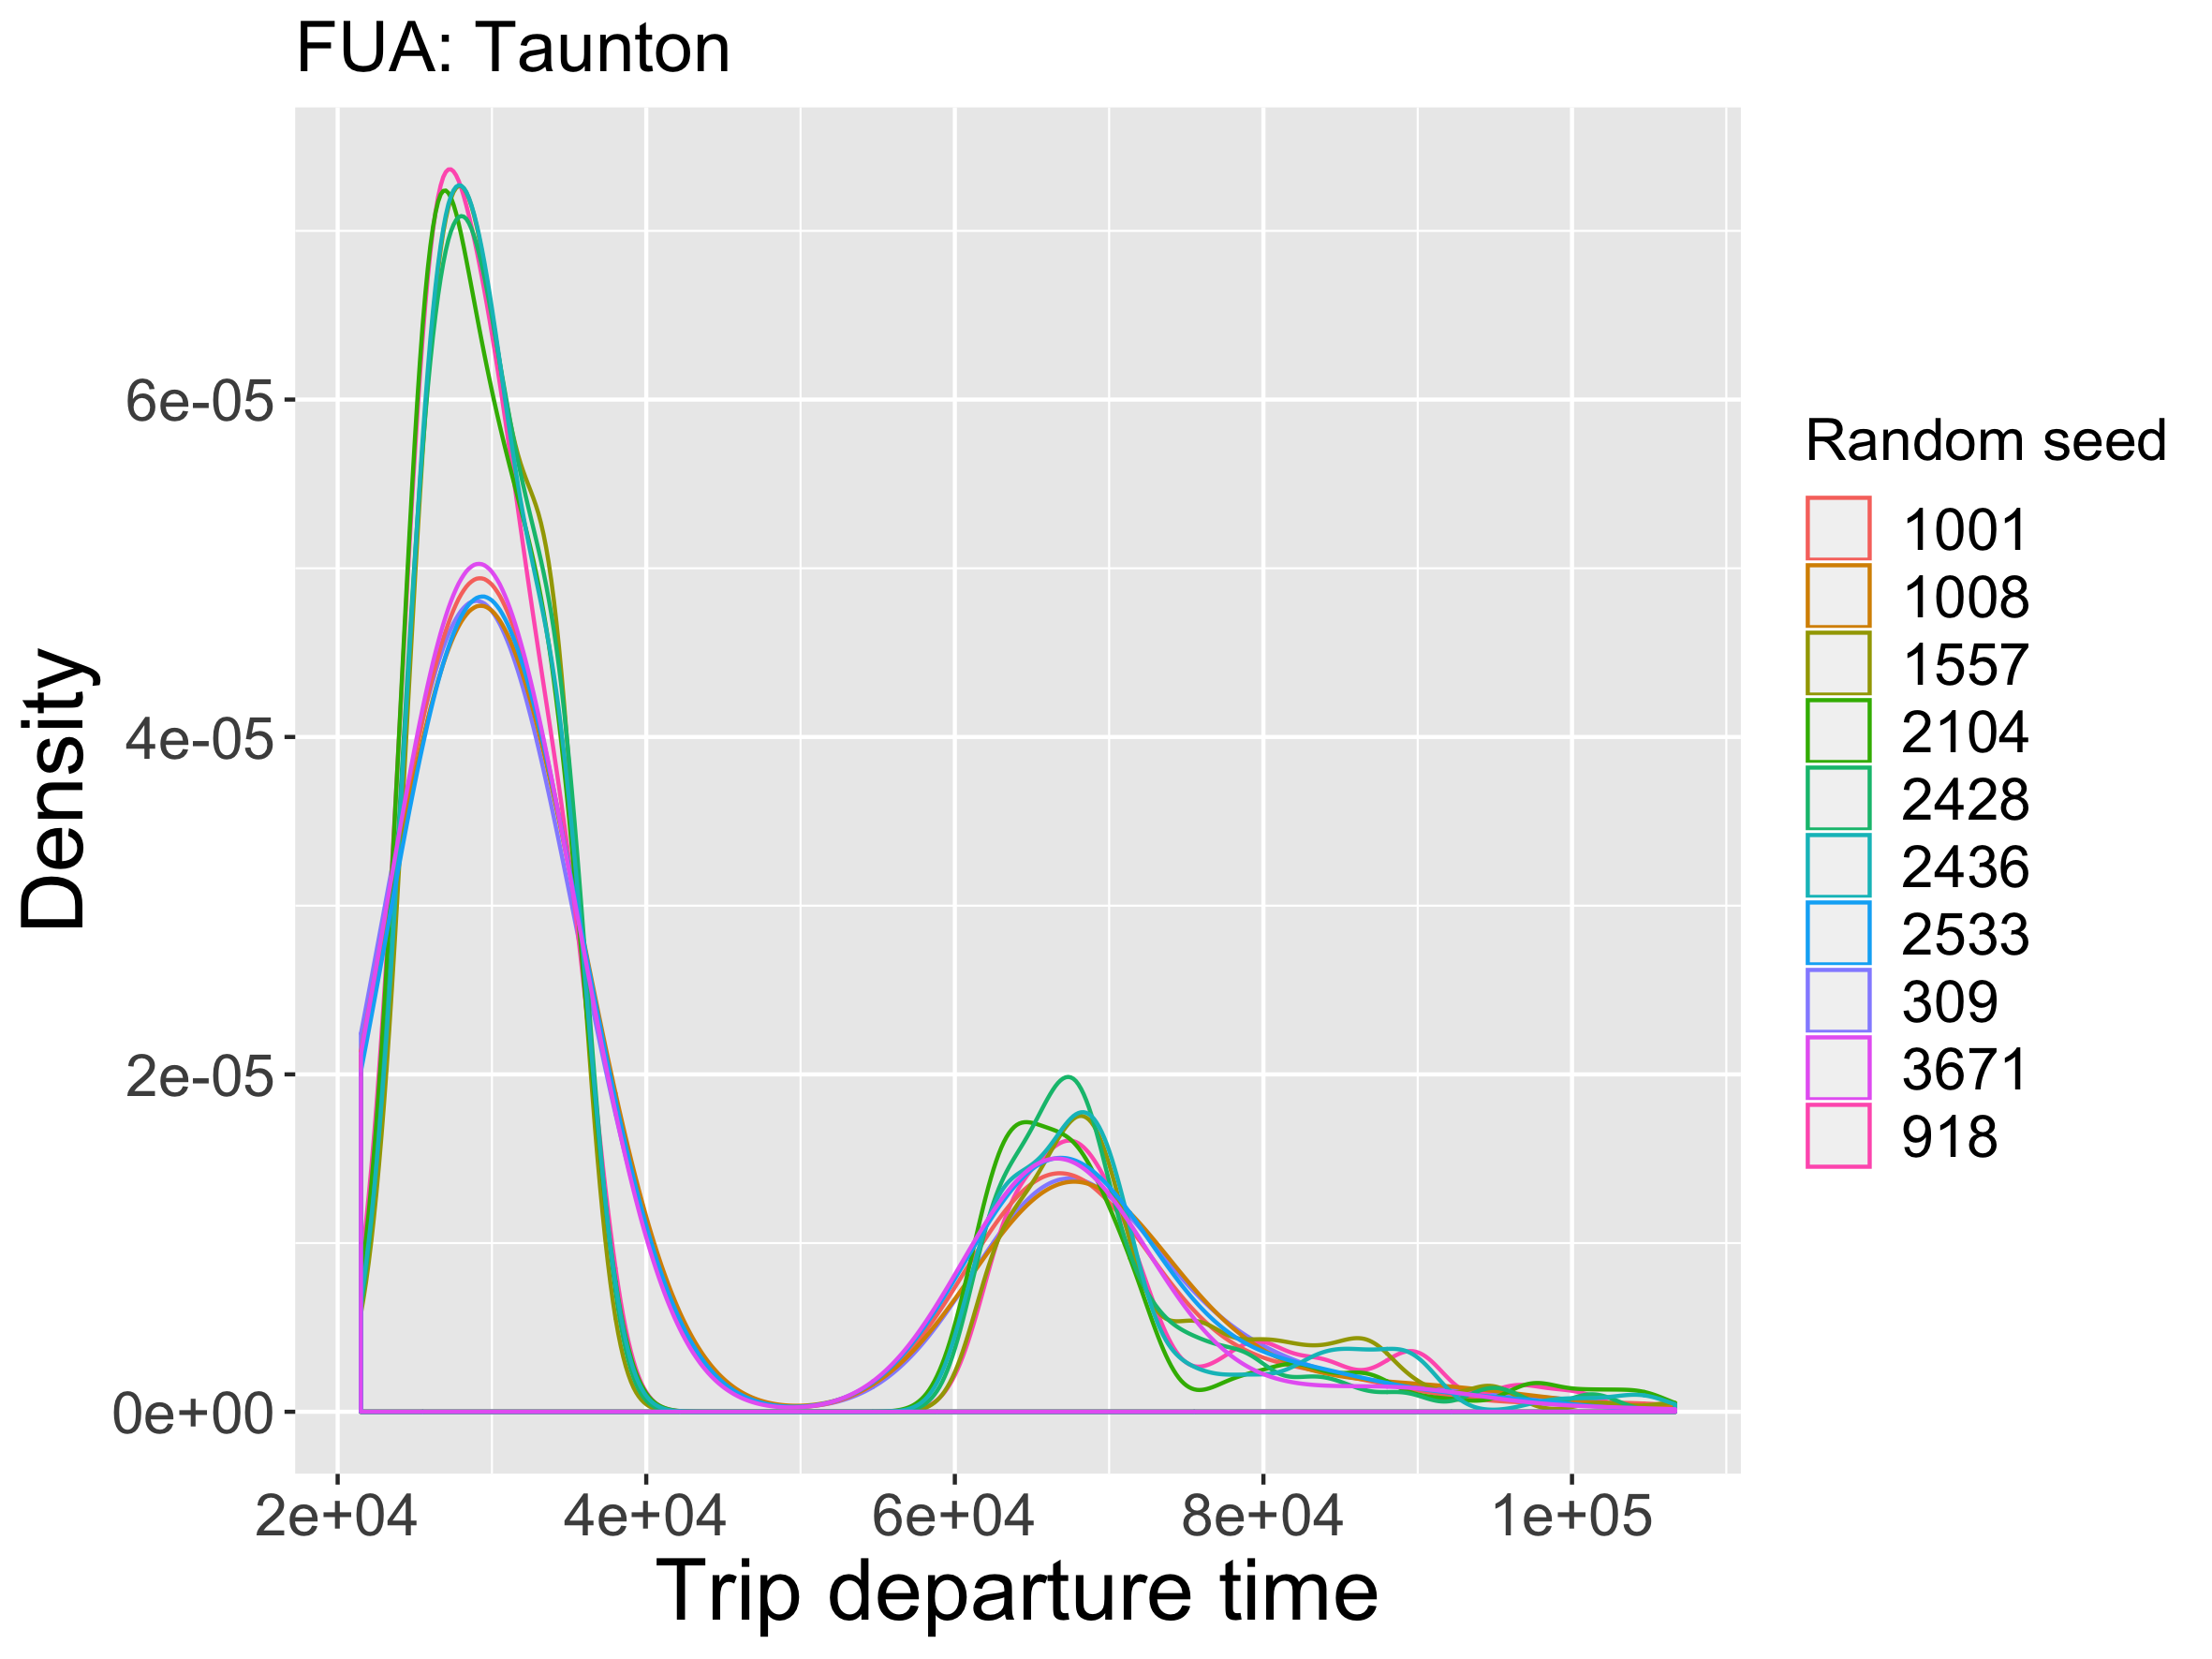
\includegraphics[width=0.48\linewidth]{figures/stochasticity_Taunton.png}	
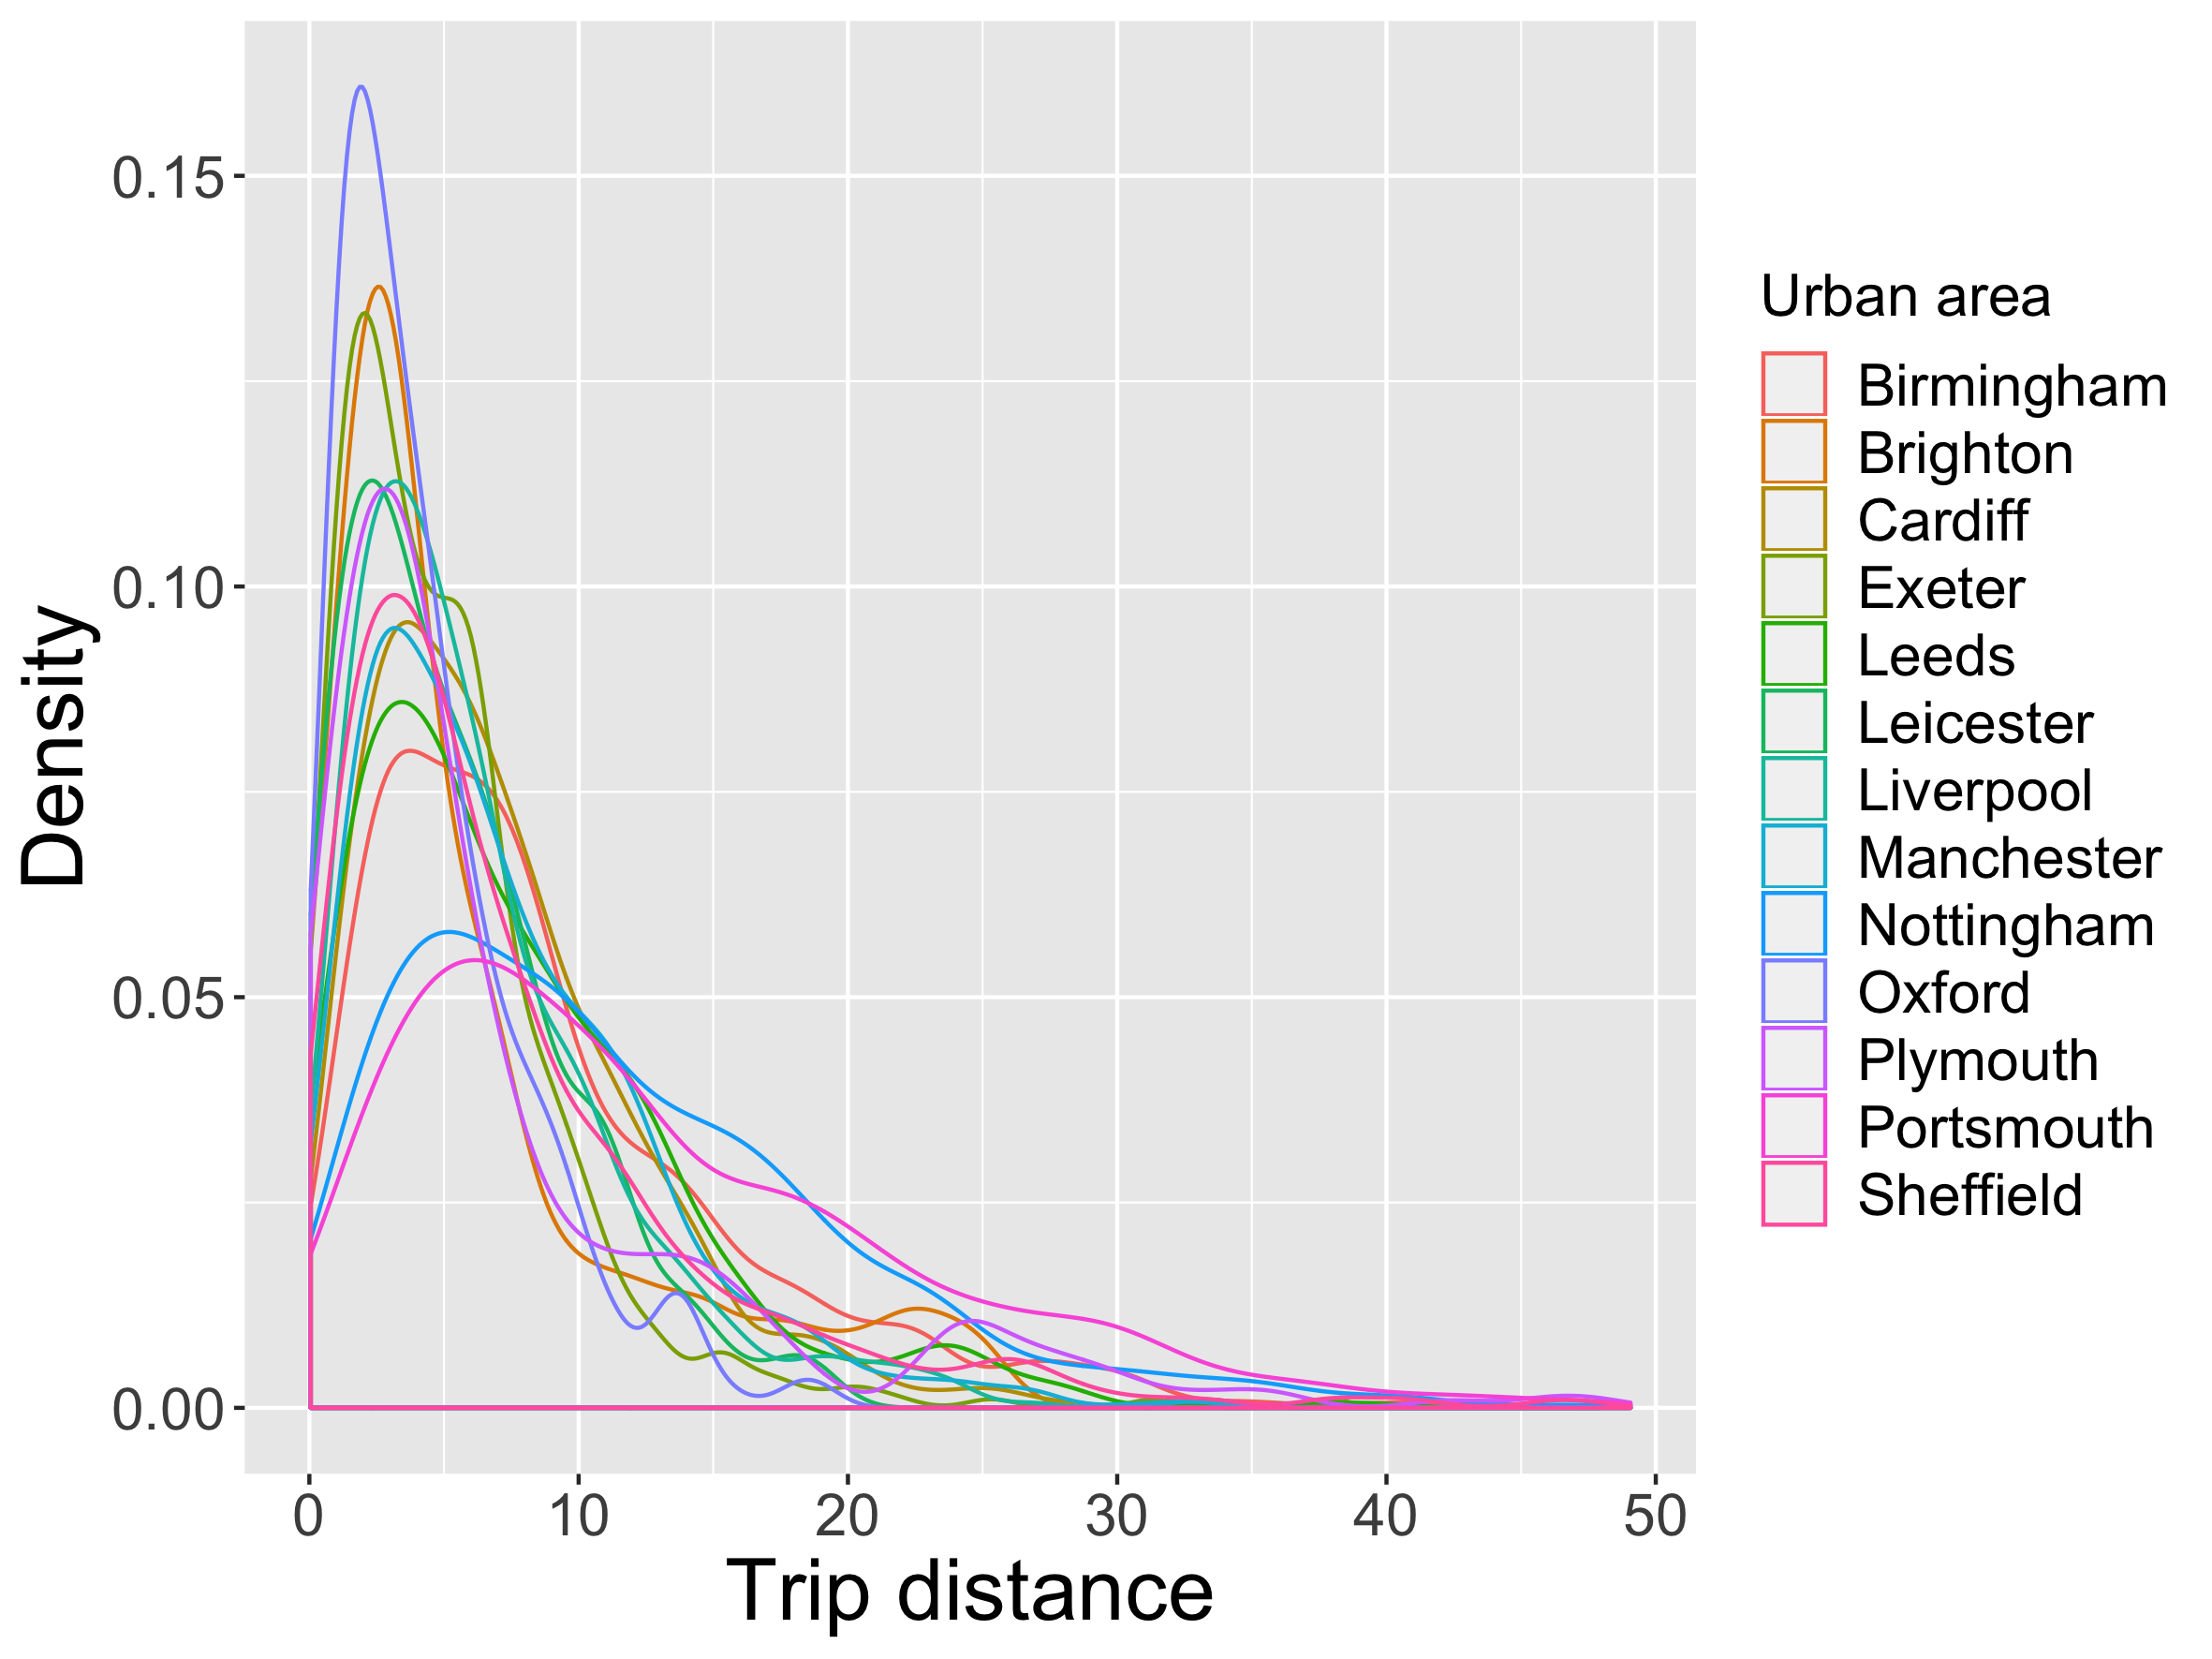
\includegraphics[width=0.48\linewidth]{figures/distances_allFUAs.png}
\end{center}
\caption{Results of the simulation of the integrated model on the largest functional urban areas in the UK. \textit{(Left)} Distribution of trip departure times, for several stochastic repetitions on the same urban area; \textit{(Right)} Distribution of trip distances for all urban areas.\label{fig:fig2}}
\end{figure}
%%%%%%%%%%%%


Source code to prepare the model components, input data, and docker containers is available on an open-source git repository at \url{https://github.com/JusteRaimbault/UrbanDynamics}.
 

To illustrate the reproducibility of our approach, we test the construction of the model with the OpenMOLE workflow engine \citep{reuillon2013openmole}, which provides a scripted workflow engine and methods to calibrate and validate simulation models, and suggest advanced numerical experiments for the validation of the coupled model. For example, studying the role of spatial configuration on model outcomes \citep{raimbault2019space} would be relevant to understand the influence of missing or imprecise data and sampling for the synthetic population.


Work in progress includes the application of this model to the development of health indicators within public transportation, and more particularly linking transportation and work-from-home policies with effective densities in public transport which provide potential exposure indicators in the context of the COVID-19 crisis.

\cite{chang2021mobility}








%\section{Discussion}


%% References
%%
%% Following citation commands can be used in the body text:
%% Usage of \cite is as follows:
%%   \cite{key}         ==>>  [#]
%%   \cite[chap. 2]{key} ==>> [#, chap. 2]
%%

%The citation must be used in following style: \cite{article-minimal} \cite{article-full} \cite{article-crossref} \cite{whole-journal}.
%% References with BibTeX database:

%
\newpage

\bibliographystyle{elsarticle-harv}
\bibliography{biblio.bib}

\clearpage


\end{document}

%%%%
% Template

%
%\begin{figure}[t]\vspace*{4pt}
%%\centerline{\includegraphics{fx1}\hspace*{5mm}\includegraphics{fx1}}
%\centerline{\includegraphics{gr1}}
%\caption{(a) first picture; (b) second picture.}
%\end{figure}
%
%\begin{table}[h]
%\caption{An example of a table.}
%\begin{tabular*}{\hsize}{@{\extracolsep{\fill}}lll@{}}
%\toprule
%An example of a column heading & Column A ({\it{t}}) & Column B ({\it{t}})\\
%\colrule
%And an entry &   1 &  2\\
%And another entry  & 3 &  4\\
%And another entry &  5 &  6\\
%\botrule
%\end{tabular*}
%\end{table}
%



%
%\begin{equation}
%\begin{array}{lcl}
%\displaystyle X_r &=& \displaystyle\dot{Q}^{''}_{rad}\left/\left(\dot{Q}^{''}_{rad} + \dot{Q}^{''}_{conv}\right)\right.\\[6pt]
%\displaystyle \rho &=& \displaystyle\frac{\vec{E}}{J_c(T={\rm const.})\cdot\left(P\cdot\left(\displaystyle\frac{\vec{E}}{E_c}\right)^m+(1-P)\right)}
%\end{array}
%\end{equation}
%
%



%% The Appendices part is started with the command \appendix;
%% appendix sections are then done as normal sections
%% \appendix

%% \section{}
%% \label{}
%
%\appendix
%\section{An example appendix}
%Authors including an appendix section should do so before References section. Multiple appendices should all have headings in the style used above. They will automatically be ordered A, B, C etc.
%
%\subsection{Example of a sub-heading within an appendix}
%There is also the option to include a subheading within the Appendix if you wish.
%



%
%
%\section*{Acknowledgements}
%
%Acknowledgements and Reference heading should be left justified, bold, with the first letter capitalized but have no numbers. Text below continues as normal.
%

